\begin{table}
\centering
%\small
\caption{Results of ER for Onemax.}
\begin{tabular}{|r|r|rr|rr|}
\hline
\multicolumn{1}{|c|}{N} & \multicolumn{1}{|c|}{c} & 
\multicolumn{2}{c|}{Best} & \multicolumn{2}{c|}{Evaluations} \\ \hline
100 & 0.1 & --397.4 &  (1.5) & 3409 &  (83.72) \\ \hline
500 & 0.1 & --400 &  (0) & 15500 &  (196.21) \\ \hline
1000 & 0.1 & --400 &  (0) & 30300 &  (788.67) \\ \hline
3000 & 0.1 & --400 &  (0) & 90300 &  (1728.58) \\ \hline
100 & 0.3 & --397.4 &  (0.92) & 3103 &  (86.38) \\ \hline
500 & 0.3 & --400 &  (0) & 14045 &  (260.24) \\ \hline
1000 & 0.3 & --400 &  (0) & 28030 &  (283.02) \\ \hline
3000 & 0.3 & --400 &  (0) & 82200 &  (1505.99) \\ \hline
100 & 0.5 & --397.1 &  (0.83) & 2750 &  (100) \\ \hline
500 & 0.5 & --400 &  (0) & 12650 &  (165.83) \\ \hline
1000 & 0.5 & --400 &  (0) & 24750 &  (460.98) \\ \hline
3000 & 0.5 & --400 &  (0) & 74100 &  (994.99) \\ \hline
100 & 0.7 & --394.5 &  (2.2) & 2397.7 &  (75.9) \\ \hline
500 & 0.7 & --400 &  (0) & 11004.9 &  (104.7) \\ \hline
1000 & 0.7 & --400 &  (0) & 21410.8 &  (523.08) \\ \hline
3000 & 0.7 & --400 &  (0) & 62401.7 &  (1639.37) \\ \hline
\end{tabular}
\label{result_0d_idea}
\end{table}

\begin{table}
\centering
\caption{Results of RTR ($C=0.7$) for Onemax.}
\begin{tabular}{|r|r|rr|rr|}
\hline
\multicolumn{1}{|c|}{N} & \multicolumn{1}{|c|}{M} & 
\multicolumn{2}{c|}{Best} & \multicolumn{2}{c|}{Evaluations} \\ \hline
10 & 10 & --255.9 &  (7.44) & 193 &  (16.16) \\ \hline
50 & 10 & --331.7 &  (5.9) & 2900010 &  (0) \\ \hline
50 & 50 & --370.9 &  (4.91) & 2900050 &  (0) \\ \hline
100 & 10 & --372.6 &  (4.78) & 2900010 &  (0) \\ \hline
100 & 50 & --390.1 &  (2.12) & 2900050 &  (0) \\ \hline
100 & 100 & --397.1 &  (1.81) & 2610730 &  (868110) \\ \hline
200 & 10 & --398.1 &  (1.22) & 2610823 &  (867561) \\ \hline
200 & 50 & --399 &  (0.89) & 2032990 &  (1324456.48) \\ \hline
200 & 100 & --399.7 &  (0.46) & 878810 &  (1323251.13) \\ \hline
200 & 200 & --400 &  (0) & 10820 &  (3552.41) \\ \hline
300 & 10 & --400 &  (0) & 18704 &  (3981.81) \\ \hline
300 & 50 & --399.9 &  (0.3) & 308135 &  (863982.34) \\ \hline
300 & 100 & --400 &  (0) & 18650 &  (2154.65) \\ \hline
300 & 200 & --400 &  (0) & 17320 &  (1695.76) \\ \hline
300 & 300 & --400 &  (0) & 18600 &  (2212.69) \\ \hline
\end{tabular}
\label{result_0d_rtr}
\end{table}

\vspace{0.5cm}

\begin{table}[tb]
\centering
\caption{Results of RPM ($C=0.01$) for Onemax.}
%\small
\begin{tabular}{|r|r|rr|rr|}
\hline
\multicolumn{1}{|c|}{N} & \multicolumn{1}{|c|}{M} & 
\multicolumn{2}{c|}{Best} & \multicolumn{2}{c|}{Evaluations} \\ \hline
10 & 10 & --267.8 &  (8.82) & 1455 &  (197.7) \\ \hline
50 & 10 & --395.7 &  (1.73) & 17935 &  (1268.47) \\ \hline
50 & 50 & --399.9 &  (0.3) & 118075 &  (4346.22) \\ \hline
100 & 10 & --400 &  (0) & 20291 &  (341.86) \\ \hline
100 & 50 & --400 &  (0) & 133730 &  (4321.41) \\ \hline
100 & 100 & --400 &  (0) & 313720 &  (9888.26) \\ \hline
200 & 10 & --400 &  (0) & 30225 &  (437.16) \\ \hline
200 & 50 & --400 &  (0) & 210360 &  (4185.08) \\ \hline
200 & 100 & --400 &  (0) & 476680 &  (8545.62) \\ \hline
200 & 200 & --398.8 &  (3.28) & 1040020 &  (122154.02) \\ \hline
300 & 10 & --400 &  (0) & 29187 &  (343.77) \\ \hline
300 & 50 & --400 &  (0) & 281865 &  (3792.63) \\ \hline
300 & 100 & --400 &  (0) & 609900 &  (11553.87) \\ \hline
300 & 200 & --400 &  (0) & 1319380 &  (23383.96) \\ \hline
300 & 300 & --397.3 &  (6.87) & 2019090 &  (315916.21) \\ \hline
\end{tabular}
\label{result_0d_rpm}
\end{table}

\begin{table}[tb]
%\small
\centering
\caption{The 5 best cases of RTR for 1D and 2D Ising. In all cases, the
 population does not converge and thus $2.9\times 10^6$ function
 evaluations are performed.}

(a) 1D Ising\\
\begin{tabular}{|r|r|r|rr|}
\hline
\multicolumn{1}{|c|}{N} & \multicolumn{1}{|c|}{M} & 
\multicolumn{1}{c|}{c} & \multicolumn{2}{c|}{Best} \\ \hline
200 & 200 & 0.3 & --370.2 & (5.55) \\ \hline
500 & 10 & 0.7 & --369.8 & (2.89) \\ \hline
200 & 10 & 0.3 & --369.6 & (3.07) \\ \hline
300 & 10 & 0.5 & --369.4 & (3.35) \\ \hline
500 & 500 & 0.7 & --369 & (3.13) \\ \hline
\end{tabular}

%\label{}
%\end{table}

\vspace{0.5cm}

%\begin{table}[tb]
(b) 2D Ising\\
\begin{tabular}{|r|r|r|rr|}
\hline
\multicolumn{1}{|c|}{N} & \multicolumn{1}{|c|}{M} & 
\multicolumn{1}{c|}{c} & \multicolumn{2}{c|}{Best} \\ \hline
500 & 300 & 0.7 & --733.4 & (9.96) \\ \hline
200 & 10 & 0.3 & --731.8 & (18.41) \\ \hline
200 & 100 & 0.3 & --729.8 & (14.52) \\ \hline
200 & 50 & 0.3 & --729 & (7) \\ \hline
300 & 50 & 0.5 & --728.2 & (11.15) \\ \hline
\end{tabular}
\label{table_rtr_1d_2d}
\end{table}

\begin{table}
\centering
\caption{The results of RPM ($N=500, c=0.01$) for 1D and 2D Ising.}
(a) 1D Ising\\
\begin{tabular}{|r|rr|rr|}
\hline
\multicolumn{1}{|c|}{M} &  \multicolumn{2}{c|}{Best} 
& \multicolumn{2}{c|}{Evaluations} \\ \hline
10 & --367.6 &  (2.5) & 33113 &  (1197.29) \\ \hline
50 & --376.4 &  (4.18) & 212620 &  (6956.98) \\ \hline
100 & --379.2 &  (2.99) & 426020 &  (17388.26) \\ \hline
200 & --379.6 &  (3.77) & 870180 &  (23316.64) \\ \hline
300 & --379.2 &  (3.92) & 1336070 &  (48353.53) \\ \hline
400 & --381.6 &  (4.54) & 1867220 &  (57325.4) \\ \hline
500 & --382.4 &  (2.94) & 2365300 &  (93769.45) \\ \hline
\end{tabular}

\vspace{0.5cm}

(b) 2D Ising\\
\begin{tabular}{|r|rr|rr|}
\hline
\multicolumn{1}{|c|}{M} &  \multicolumn{2}{c|}{Best} 
& \multicolumn{2}{c|}{Evaluations} \\ \hline
10 & --724.8 & (14.29) & 39582 & (1398.18) \\ \hline
50 & --738.8 & (11.32) & 230640 & (9368.96) \\ \hline
100 & --749.4 & (8.81) & 494280 & (20965.72) \\ \hline
200 & --766.4 & (12.64) & 1186340 & (92668.69) \\ \hline
300 & --749.2 & (6.34) & 1742000 & (40892.32) \\ \hline
400 & --761.6 & (15.89) & 2473260 & (146213.15) \\ \hline
500 & --761.4 & (18.11) & 2900500 & (0) \\ \hline
\end{tabular}
\label{table_rpm_1d_2d}
\end{table}

\begin{figure}[tb]
%\centering
\centerline{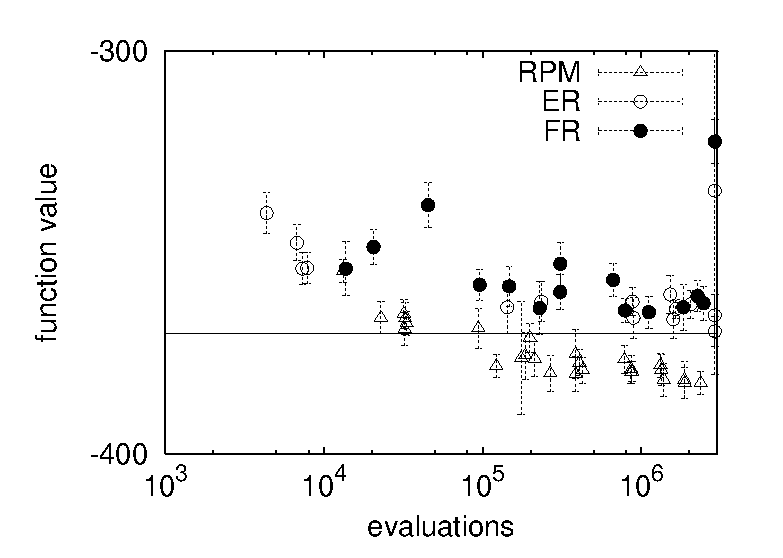
\includegraphics[width=\figlength\linewidth]{data_rpm/idea_vs_rwor_1d.eps}}
\caption{Results for 1D Ising.}
\label{result_1d}
%\end{figure}

\vspace{0.5cm}

%\begin{figure}[tb]
\centerline{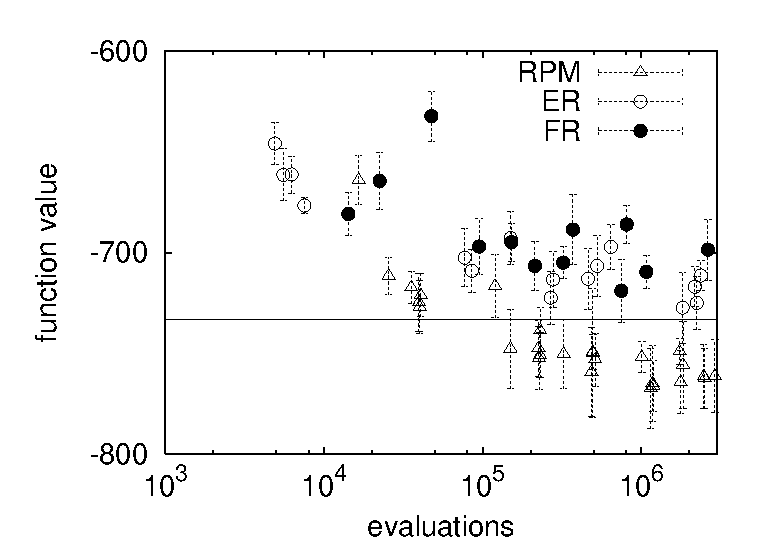
\includegraphics[width=\figlength\linewidth]{data_rpm/idea_vs_rwor_2d.eps}}
\caption{Results for 2D Ising.}
\label{result_2d}
\end{figure}

%\vspace{0.5cm}

\begin{figure}[tb]
\centerline{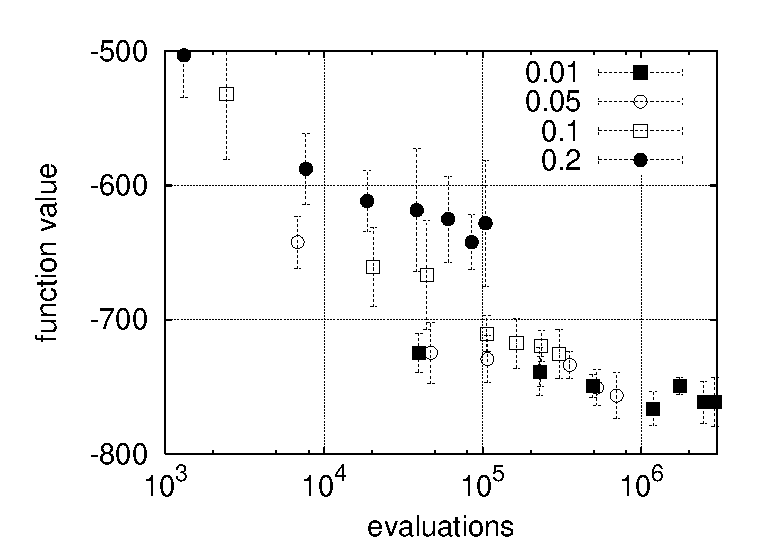
\includegraphics[width=\figlength\linewidth]{data_rpm/rpm_rwor_2d_cutoff.eps}}
\caption{Results of RPM ($N=500$) for 2D Ising.}
\label{result_cutoff}
\end{figure}

